\documentclass[12pt,a4paper]{article}

\usepackage{wrapfig}
\usepackage{graphicx}
\usepackage[T1]{fontenc}
\usepackage[polish]{babel}
\usepackage[utf8]{inputenc}
\usepackage[font=footnotesize,labelfont=bf]{caption}


\usepackage[
    backend=biber,
    sorting=ynt
]{biblatex}
\addbibresource{draft.bib}

\title{Bibliography management: \texttt{biblatex} package}

\author{Krzytsztof Wiśniewski}
\date{ }

\begin{document}


\begin{titlepage}
    \centering

    \Large
    \textbf{UNIWERSYTET GDAŃSKI}\\
    \textbf{WYDZIAŁ MATEMATYKI, FIZYKI I INFORMATYKI}

    \vspace{2.5cm}

    \large
    \textbf{Krzysztof Wiśniewski}\\
    \textbf{numer albumu: 274276}

    \vspace{1.5cm}
    \raggedright
    \small
    Kierunek studiów: Bioinformatyka\\
    Specjalność: Ogólna

    \vspace{1.5cm}

    \centering
    \Large
    \textbf{Optymalizacja oprogramowania w języku Python do analizy stanów kwantowych.}

    \vfill

    \raggedleft
    \normalsize
    Praca licencjacka\\
    wykonana\\
    pod kierunkiem\\
    dr hab. Marcin Wieśniak, prof. UG\\

    \vfill

    \centering
    \large
    Gdańsk 2023

\end{titlepage}
\newpage

\tableofcontents
\newpage

\begin{sloppypar}

    \begin{abstract}
        W tej pracy przeprowadzam analizę możliwości optymalizacji pod kątem czasu wykonania
        oprogramowania napisanego w języku Python przez pryzmat programu CSSFinder służącego
        do analizy stanów kwantowych pod kątem detekcji splątania kwantowego. Pośród rozważanych
        metod obecna będzie standardowa implementacja w języku Python z wykorzystaniem
        biblioteki NumPy\cite{NumPy_Article}\cite{NumPy_Doc}, wersja wzbogacona o
        kompilację JIT przy pomocy biblioteki Numba\cite{Numba_Article}\cite{Numba_Doc},
        wersja skompilowana do kodu maszynowego przy pomocy biblioteki Cython i GCC oraz
        implementacja w języku Rust, również skompilowana do kodu maszynowego.

    \end{abstract}

    \section[wstęp]{Wstęp}

    Język Python zachęca użytkowników prostotą składni, łatwością tworzenia kodu, ze względu
    na swoją dynamiczną naturę i automatyczne zarządzanie pamięcią, mnogością dostępnych
    bibliotek otwartoźródłowych, czy rozbudowaną społecznością programistów.
    Niestety, wygoda i elastyczność tego języka ma pewien ukryty koszt. Interpretowany
    kod, napisany w Pythonie, pod względem wydajności znacząco odstaje od kompilowanych
    języków programowania (C, Fortran, C++, Rust). Istnieją jednakże metody pozwalające
    na obejście tej niedogodności.

    \begin{figure}[h]
        \centering
        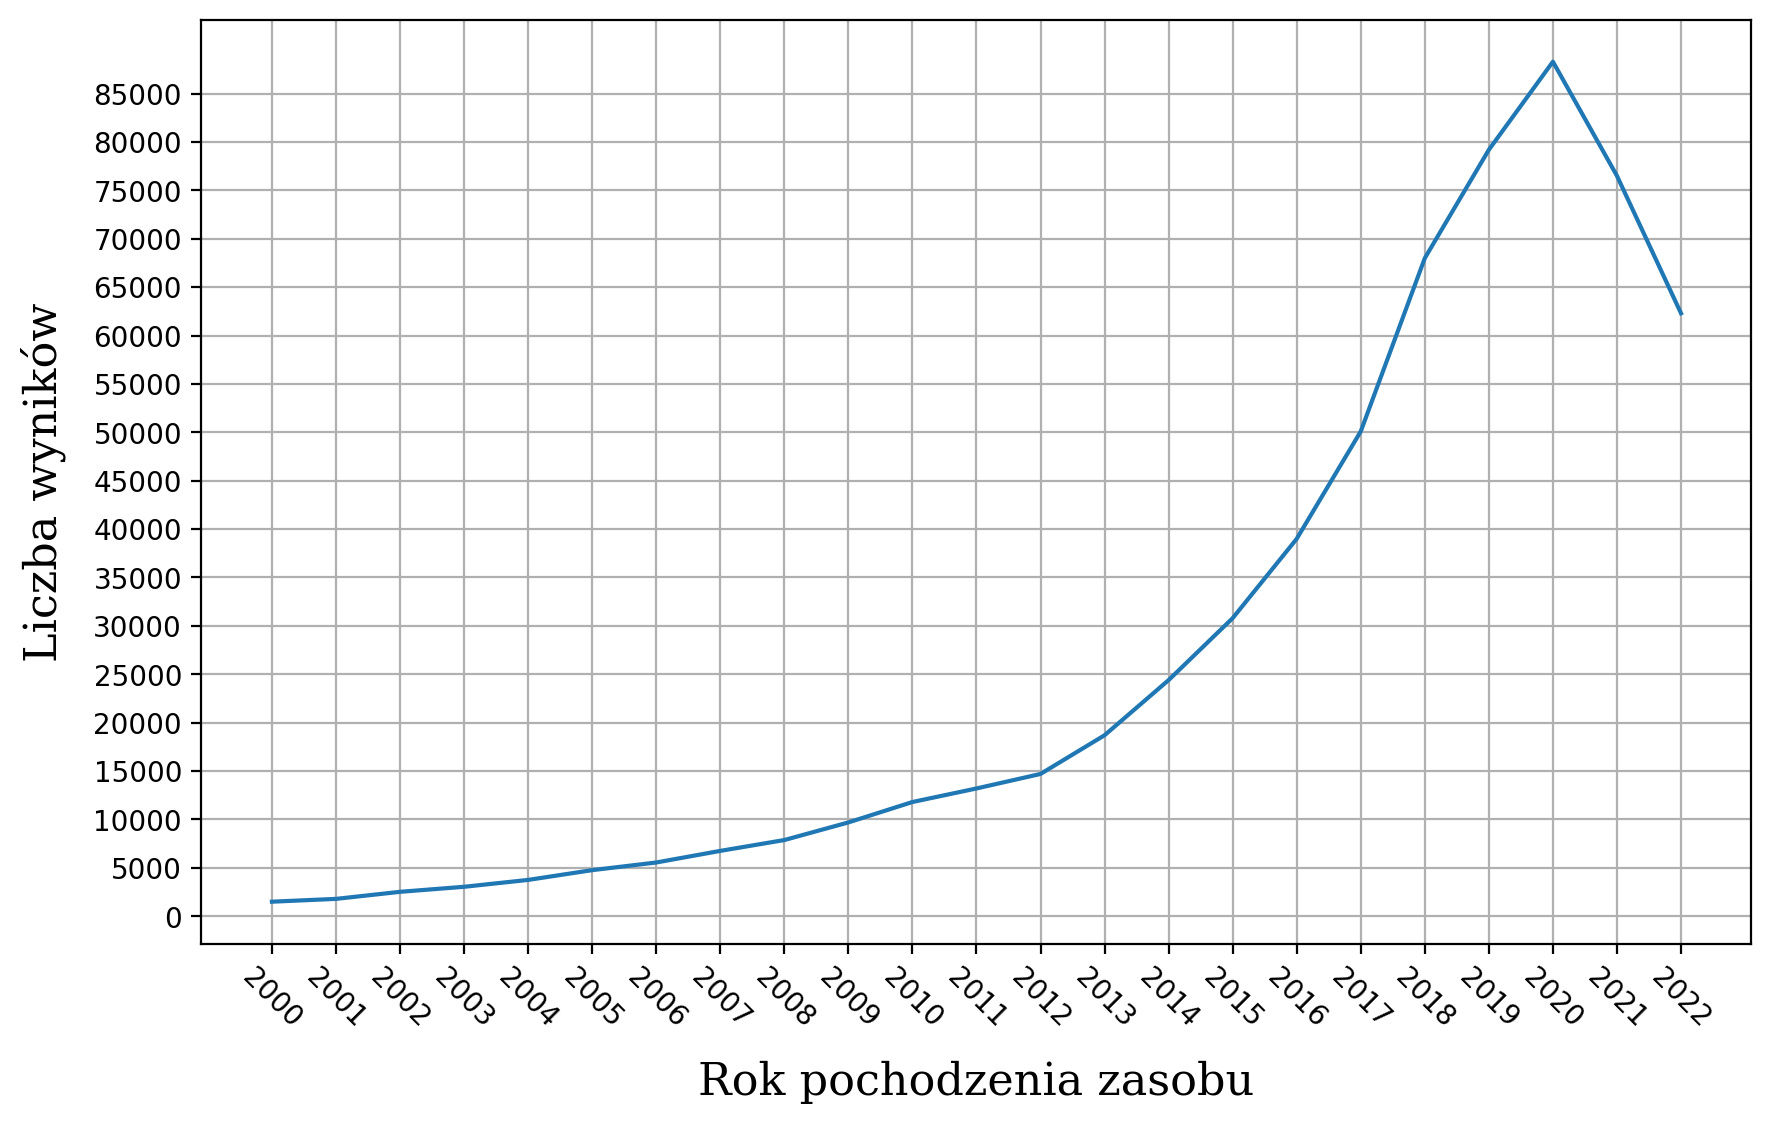
\includegraphics[width=0.8\textwidth]{"images/python_language_results.png"}
        \caption{Ilość wyników Google Scholar dla zapytania 'python language' z podziałem na rok wydania}
    \end{figure}

    \subsection{Cel pracy}

    Praca ma na celu rozpatrzenie efektów uzyskiwanych różnymi sposobami optymalizacji kodu
    w przypadku konkretnego oprogramowania. Analizy dotyczyć będą programu CSSFinder którego
    wielokrotnej re-implementacji, z wykorzystaniem różnych metod optymalizacji, dokonałem
    w ramach prac projektowych. Wraz z optymalizacją udoskonalony został interfejs użytkownika
    programu, a sam wynikowy kod dostępny jest na GitHub'ie\cite{CSSFinder_New}\cite{CSSFinder_New_Numpy}\cite{CSSFinder_New_Rust}.

    \subsection{Biblioteki współdzielone}

    Klasycznym
    rozwiązaniem jest ucieknięcie się do wykorzystania odpowiednio spreparowanych narzędzi
    napisanych w językach niższego poziomu (C, C++, Rust i potencjalnie inne), które
    interpreter jest w stanie zaimportować.  Mamy więc w tym wypadku do czynienia z
    kompilacją przed czasem wykonywania (ahead-of-time compilation - AOT compilation).
    Pozwala to na utworzenie zbioru relatywnie prymitywnych narzędzi w językach wymagających
    więcej czasu i pracy, aby następnie komponować je w skompilowane oprogramowanie
    w języku wielokrotnie prostszym. Przykładami takich bibliotek są NumPy oraz CuPy.
    Pierwsza z nich koncentruje się na obliczeniach wykonywanych na CPU, druga jest
    bliźniaczo podobna, ale wykorzystuje GPU.

    \subsection{Kompilacja JIT}

    Możliwości przyspieszania Pythona nie kończą się na pisaniu kodu w innych językach.
    Dzięki odpowiednim narzędziom wykonalne jest podążenie w ślady języków takich jak
    JavaScrip, Lua czy Java i wykorzystanie kompilacji do kodu maszynowego w czasie
    wykonywania (just-in-time compilation - JIT compilation).
    W momencie pisania tej pracy istnieją dwa szeroko dostępne narzędzia oferujące
    kompilację JIT. Pierwszym jest biblioteka Numba, która pozwala na kompilację
    odpowiednio oznaczonych fragmentów kodu. Drugą jest pełna alternatywna implementacja
    interpretera Pythona, PyPy, która automatycznie decyduje które fragmenty kodu
    skompilować.

    \subsection{Cython}

    Rozwiązaniem pomiędzy uprzednio wymienionymi jest Cython. Jest to zarówno nazwa
    biblioteki jak i nadzbioru języka Python który pozwala na dodatkowe adnotowanie kodu
    informacjami o typach. Kod napisany w Cythonie można następnie transpilować do C
    lub C++ po czym skompilować do kodu maszynowego. Cython nie wymaga aby w
    kompilowanym kodzie znajdowały się dodatkowe adnotacje, wzwiązku z czym możliwe jest
    skompilowanie czystego kodu Pythona do kodu maszynowego. Pozwala to na pozbycie się
    obciążenia ze strony procesu interpretacji i oraz skorzystać z optymalizacji które
    potrafią wykonywać współczesne kompilatory. Nie usuwa to jednak obciążenia ze strony
    dynamicznego systemu typów, czyniąc kompilację bez adnotacji mało efektywną.

    \subsection{}

\end{sloppypar}

\newpage
\begin{sloppypar}
    \medskip

    \printbibliography[
        heading=bibintoc,
        title={Źródła}
    ]

\end{sloppypar}

\end{document}